\documentclass[zihao=false,fontset=windows]{ctexart}
% ctexart 不接受任意 pt 选项。正文改 {10pt}，方括号里是行距。
\usepackage{scrextend}
\usepackage{needspace}
\changefontsizes[12pt]{10pt}

\usepackage[a4paper,left=2.35cm,right=2.35cm,top=1.7cm,bottom=1.9cm]{geometry}
\usepackage{xcolor}
\usepackage{graphicx}
\usepackage{amsmath,amssymb}
\usepackage{enumitem}
\usepackage{tabularx}
\usepackage{colortbl}
\usepackage{listings}
\usepackage{hyperref}
\usepackage[most]{tcolorbox}

\definecolor{feishuText}{RGB}{31,35,41}
\definecolor{feishuBlue}{RGB}{36,91,219}
\definecolor{feishuRed}{RGB}{216,57,49}
\definecolor{feishuGray}{RGB}{100,106,115}
\definecolor{feishuGray2}{RGB}{143,149,158}
\definecolor{feishuPinkBg}{RGB}{251,191,188}
\definecolor{quoteBar}{RGB}{51,112,255}
\definecolor{codebg}{RGB}{245,246,247}
\definecolor{codeborder}{RGB}{222,224,227}
\definecolor{inlinebg}{RGB}{242,243,245}
\definecolor{callRed}{RGB}{253,226,226}
\definecolor{callOrange}{RGB}{255,245,235}
\definecolor{callYellow}{RGB}{254,255,240}
\definecolor{callGreen}{RGB}{240,251,239}
\definecolor{callBlue}{RGB}{240,244,255}
\definecolor{callRedSoft}{RGB}{254,241,241}
\definecolor{callSun}{RGB}{255,255,204}
\definecolor{tableHead}{RGB}{242,243,245}
\definecolor{tableRule}{RGB}{222,224,227}
\definecolor{codeText}{RGB}{31,35,41}
\definecolor{codeKeyword}{RGB}{0,0,255}
\definecolor{codeComment}{RGB}{0,128,0}
\definecolor{codeString}{RGB}{163,21,21}

\setmainfont{Times New Roman}
\setCJKmainfont{Microsoft YaHei}[AutoFakeBold=2.2]
\setCJKsansfont{Microsoft YaHei}[AutoFakeBold=2.2]
\setCJKmonofont{Microsoft YaHei}[AutoFakeBold=2.2]
\setmonofont{Consolas}
\newfontfamily\emojifont{Segoe UI Emoji}

\hypersetup{
  colorlinks=true,
  urlcolor=feishuBlue,
  linkcolor=feishuBlue,
  unicode=true,
  pdftitle={Qwen2-VL}
}

\setlength{\parindent}{0pt}
\setlength{\parskip}{0.42em}
\setlength{\fboxsep}{1.5pt}
\setlength{\emergencystretch}{3em}
\linespread{1.28}
\color{feishuText}
\arrayrulecolor{tableRule}
\urlstyle{same}

\setlist[enumerate]{label=\textcolor{feishuBlue}{\arabic*.}, leftmargin=1.7em, itemsep=0.22em, topsep=0.28em, parsep=0.08em, partopsep=0pt}
\setlist[itemize,1]{label=\textcolor{feishuBlue}{\textbullet}, leftmargin=1.35em, itemsep=0.18em, topsep=0.25em, parsep=0.06em, partopsep=0pt}
\setlist[itemize,2]{label=\textcolor{feishuBlue}{◦}, leftmargin=1.45em, itemsep=0.12em, topsep=0.15em}
\setlist[itemize,3]{label=\textcolor{feishuBlue}{\rule[0.18em]{0.38em}{0.38em}}, leftmargin=1.55em, itemsep=0.1em, topsep=0.12em}

\newcommand{\feiEmoji}[1]{{\emojifont #1}}
\newcommand{\incode}[1]{\colorbox{inlinebg}{\ttfamily\small #1}}
\newcommand{\bigmath}[1]{%
  \begin{center}\large$\displaystyle #1$\end{center}%
}

\lstset{
  language=Python,
  basicstyle=\ttfamily\footnotesize\color{codeText},
  keywordstyle=\color{codeKeyword},
  commentstyle=\color{codeComment},
  stringstyle=\color{codeString},
  showstringspaces=false,
  breaklines=true,
  columns=fullflexible,
  keepspaces=true,
  tabsize=4,
  upquote=true,
  aboveskip=2pt,
  belowskip=0pt,
  xleftmargin=0pt,
  frame=none
}

\tcbset{
  feishubase/.style 2 args={
    enhanced,
    boxrule=0pt,
    arc=8pt,
    left=10pt,
    right=10pt,
    top=7pt,
    bottom=7pt,
    before skip=6pt,
    after skip=6pt,
    colback=#1,
    colframe=#1,
    before upper={\feiEmoji{#2}\hspace{0.45em}\ignorespaces}
  }
}
\newtcolorbox{feishubox}[2]{feishubase={#1}{#2}, breakable}
\newtcolorbox{feishuboxnb}[2]{feishubase={#1}{#2}}

\newtcolorbox{feishuquote}{
  enhanced,
  breakable,
  boxrule=0pt,
  leftrule=3pt,
  arc=0pt,
  colframe=quoteBar,
  colback=white,
  left=8pt,
  right=2pt,
  top=2pt,
  bottom=2pt,
  before skip=4pt,
  after skip=4pt,
  before upper=\color{feishuGray}
}

\newtcolorbox{feishucode}{
  enhanced,
  breakable,
  colback=codebg,
  colframe=codeborder,
  boxrule=0.6pt,
  arc=6pt,
  left=6pt,
  right=6pt,
  top=5pt,
  bottom=4pt,
  before skip=6pt,
  after skip=6pt
}


\begin{document}
{\zihao{1}\bfseries Qwen2-VL\par}
{\small\color{feishuGray} 来源：\href{https://scnajei2ds6y.feishu.cn/wiki/BHRrwQ4TAi9iCskVsMccByePngc}{飞书原文}\par}

\Needspace{5\baselineskip}\par\vspace{0.95em}\noindent{\zihao{-2}\bfseries \textcolor{feishuBlue}{1.} Architecture}\par\vspace{0.28em}

一看图片，似乎没有Adaptor存在了，难道Vision Encoder出来的特征直接就送LLM了吗？（显然不是，MLP藏在Vision Encoder里面了）\par

\begin{center}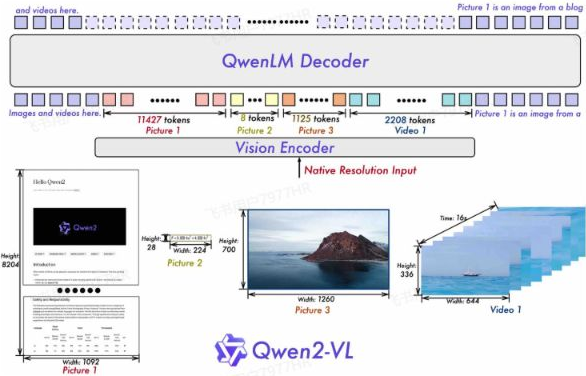
\includegraphics[width=0.82\textwidth]{images/Qwen2-VL/fig-01.png}\end{center}

\Needspace{5\baselineskip}\par\vspace{0.95em}\noindent{\zihao{3}\bfseries \textcolor{feishuBlue}{1.1} Vision Encoder}\par\vspace{0.28em}

Qwen2-VL支持动态分辨率（and视频），这一点是通过MRoPE (RoPE-2D) 实现的，也就是说扩充了允许patch的动态数量，也就自然而然支持动态分辨率了（当然，还是需要在stage-1训练时候训好VE）。\par

ViT参数从DFN-ViT(2)（用的是ViT的绝对位置编码）初始化，替换pos embedding为RoPE-2D。\par

\begin{itemize}

\item 2D-RoPE

\end{itemize}

把一维的RoPE转化为2D-RoPE，其实就是在于time轴上其实只是简单复制position embedding而已，真正维护的embedding只是在单帧图片的二维平面上：\par

那究竟是怎么实现2D的呢，主要看这句：\par

所以实际上实现的做法就是：现在有一个Pos Embedding预计算表PE，2D patch定位是(x,y)，那么我们需要的pos embedding就是PE[x],PE[y]在dim维度上concat一下。那么可能有的人会问，那维度怎么和head\_dim对上，其实就在于预计算表PE是用(head\_dim//2)来初始化的：\par

关于2D-RoPE的详细代码解析参考\href{https://scnajei2ds6y.feishu.cn/wiki/BHUIwyfVUizmwQkKQPFceqJrnEe}{2D-RoPE}\par

\Needspace{5\baselineskip}\par\vspace{0.95em}\noindent{\zihao{3}\bfseries \textcolor{feishuBlue}{1.2} Adaptor}\par\vspace{0.28em}

虽然结构图上没有Adaptor，但是Qwen实质上用了两层MLP作为Adaptor，只不过这个模块PatchMerger被放在了VE也就是Qwen2VisionTransformerPretrainedModel里面了：\par

只不过这里为了控制seqlen，在MLP之前把相邻的 2*2 个 vision token 压缩成一个(其实就是在hidden\_dim上拼接)，之后再过双层MLP (PatchMerger) 。\par

\Needspace{5\baselineskip}\par\vspace{0.95em}\noindent{\zihao{3}\bfseries \textcolor{feishuBlue}{1.3} LLM}\par\vspace{0.28em}

初始化于Qwen2[3], 参数量：\par

\begin{center}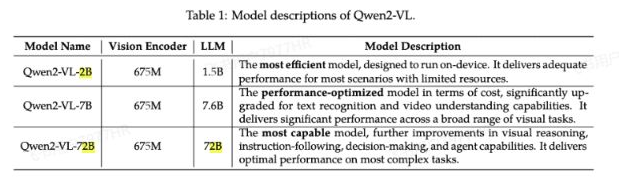
\includegraphics[width=0.90\textwidth]{images/Qwen2-VL/fig-02.png}\end{center}

\begin{itemize}

\item MRoPE

\end{itemize}

\begin{center}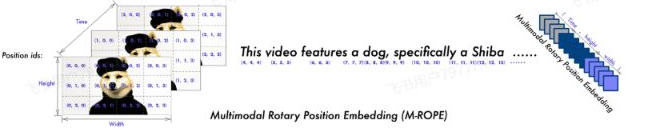
\includegraphics[width=0.98\textwidth]{images/Qwen2-VL/fig-03.png}\end{center}

MRoPE的简单示意图如上，简单理解就是pos embedding从hidden\_dim上进行了分割，分别来表示time、height、width，其实面试能答到这里已经足够了。但是秉持代码神一贯的解读代码作风，我们再来看一下具体实习，其实比上面复杂多了，参考\href{https://scnajei2ds6y.feishu.cn/wiki/JboKw8o8UiaUQbk1CBDckrtFn3f}{MRoPE}\par

\Needspace{5\baselineskip}\par\vspace{0.95em}\noindent{\zihao{-2}\bfseries \textcolor{feishuBlue}{2.} Training}\par\vspace{0.28em}

三阶段训练：\par

\begin{itemize}

\item Stage 1: 利用图像-文本对训练视觉编码器和连接层。使用了600B的token（图像分类和OCR数据）。

\item Stage 2: 训练所有参数。使用800B token。这一阶段引入更高质量的混合图像-文本内容，包含多种任务和纯文本数据。

\item Stage 3: 训练语言模型。数据包含多种任务instructional datasets、agent训练数据。

\end{itemize}

\Needspace{0.57\textheight}\par\vspace{0.95em}\noindent{\zihao{-2}\bfseries \textcolor{feishuBlue}{3.} EXP}\par\vspace{0.28em}

\begin{itemize}

\item 模型表现：

\end{itemize}

\begin{center}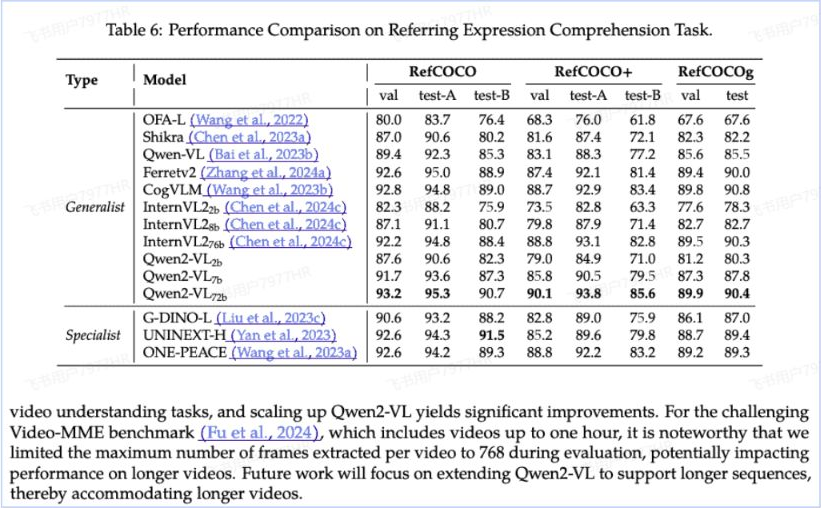
\includegraphics[width=0.85\textwidth]{images/Qwen2-VL/fig-04.png}\end{center}

\begin{itemize}

\item Ablation

\end{itemize}

MRoPE和1D-RoPE的对比：\par

\begin{center}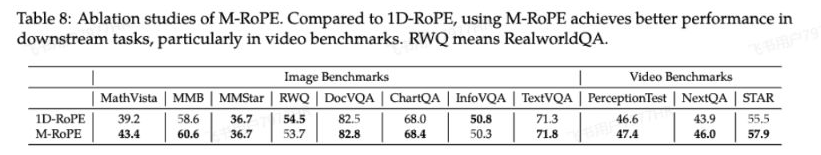
\includegraphics[width=0.98\textwidth]{images/Qwen2-VL/fig-05.png}\end{center}

以及一些比较有趣的观察，就是如果计算资源足够，那么在test-time时候做图片插值放大其实对效果是有提升的（一种Test-Time Computing的方向？）\par

\begin{center}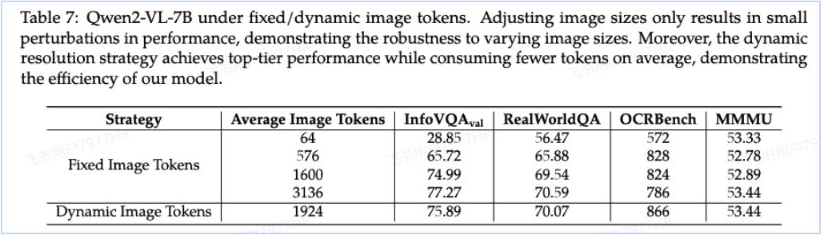
\includegraphics[width=0.92\textwidth]{images/Qwen2-VL/fig-06.png}\end{center}

\Needspace{5\baselineskip}\par\vspace{0.95em}\noindent{\zihao{-2}\bfseries \textcolor{feishuBlue}{4.} Reference}\par\vspace{0.28em}

[\textbf{1}]    Wang P, Bai S, Tan S, et al. Qwen2-vl: Enhancing vision-language model's perception of the world at any resolution[J]. arXiv preprint arXiv:2409.12191, 2024.\par

[\textbf{2}]    Fang A, Jose A M, Jain A, et al. Data filtering networks[J]. arXiv preprint arXiv:2309.17425, 2023.\par

[\textbf{3}]    Yang A, Yang B, Hui B, et al. Qwen2 technical report[J]. arXiv preprint arXiv:2407.10671, 2024.\par
\end{document}


